\documentclass[sigconf]{acmart}

\newcommand{\FIXME}[1]{{\color{red}{\textbf{FIXME:} #1}}}
\newcommand{\amdrev}[1]{{\color{blue}{#1}}}
\newcommand{\amd}[1]{{\color{blue}{[\textbf{AMD Comment:} #1]}}}
\newcommand{\lei}[1]{{\color{cyan}{[\textbf{Lei Comment:} #1]}}}
\newcommand{\hg}[1]{{\color{green}{[\textbf{Hans Comment:} #1]}}}



\usepackage{booktabs} % For formal tables

% Copyright
%\setcopyright{none}
%\setcopyright{acmcopyright}
%\setcopyright{acmlicensed}
\setcopyright{rightsretained}
%\setcopyright{usgov}
%\setcopyright{usgovmixed}
%\setcopyright{cagov}
%\setcopyright{cagovmixed}


% DOI
\acmDOI{10.475/123_4}

% ISBN
\acmISBN{123-4567-24-567/08/06}

%Conference
\acmConference[NetCompute'18]{ACM SIGCOMM 2018 Workshop on In-Network Computing conference}{August 2018}{Budapest, Hungary} 
\acmYear{2017}
\copyrightyear{2017}

\acmPrice{15.00}

\usepackage{xspace}
\newcommand{\OurSys}{Wharf\xspace}

\usepackage{algorithm2e}
\usepackage{listings}

\begin{document}
\title{In-network computing to the rescue of faulty links}
%\title{SIG Proceedings Paper in LaTeX Format}
%\titlenote{Produces the permission block, and copyright information}
%\subtitle{Extended Abstract}

\author{Hans Giesen}
\affiliation{\institution{University of Pennsylvania}}
\author{Lei Shi}
\affiliation{\institution{University of Pennsylvania}}
\author{John Sonchack}
\affiliation{\institution{University of Pennsylvania}}
\author{Anirudh Chelluri}
\affiliation{\institution{University of Pennsylvania}}
\author{Nishanth Prabhu}
\affiliation{\institution{University of Pennsylvania}}
\author{Nik Sultana}
\affiliation{\institution{University of Pennsylvania}}
\author{Latha Kant}
\affiliation{\institution{Vencore Labs}}
\author{Anthony J McAuley}
\affiliation{\institution{Vencore Labs}}
\author{Alexander Poylisher}
\affiliation{\institution{Vencore Labs}}
\author{Andr\'e DeHon}
\affiliation{\institution{University of Pennsylvania}}
\author{Boon Thau Loo}
\affiliation{\institution{University of Pennsylvania}}

%\author{Firstname Lastname}
%\authornote{Note}
%\orcid{1234-5678-9012}
%\affiliation{%
%  \institution{Affiliation}
%  \streetaddress{Address}
%  \city{City} 
%  \state{State} 
%  \postcode{Zipcode}
%}
%\email{email@domain.com}
%
%\author{Firstname Lastname}
%\orcid{1234-5678-9012}
%\affiliation{%
%  \institution{Affiliation}
%  \streetaddress{Address}
%  \city{City} 
%  \state{State} 
%  \postcode{Zipcode}
%}
%\email{email@domain.com}
%
%\author{Firstname Lastname}
%\orcid{1234-5678-9012}
%\affiliation{%
%  \institution{Affiliation}
%}
%\email{email@domain.com}
%
%\author{Firstname Lastname}
%\orcid{1234-5678-9012}
%\affiliation{%
%  \institution{Affiliation}
%}
%\email{email@domain.com}
%
%\author{Firstname Lastname}
%\orcid{1234-5678-9012}
%\affiliation{%
%  \institution{Affiliation}
%}
%\email{email@domain.com}


% The default list of authors is too long for headers}
%\renewcommand{\shortauthors}{F. Lastname et al.}
\renewcommand{\shortauthors}{H. Giesen et al.}

\begin{abstract}
Failing network links are usually disabled, and packets are routed around them
until the links are repaired. While
it is often possible
to utilize some of a failing link's capacity, losing
what remains of a link's
capacity is typically deemed preferable to the erratic effect that unreliable links can
have on application-level behavior.

We describe a new network function that relies on in-network computing to limit
the erratic effect of failing network links, to enable the continued use of
those links until they can be repaired.
%We argue that such a network function can help mitigate rolling
%failures in datacenter networks, and that our design can interoperate
%with existing network architecture and configuration choices, such as
%for multi-path routing.

We explore the design space using ns-3, and evaluate our
implementation on a physical test-bed that includes programmable
switches and reconfigurable hardware.
Our current hardware prototype uses around 10\% of our FPGA's
resources while operating at \FIXME{30\%} of its maximum clock rate,
but can almost saturate a 10GbE link.
\hg{The current frequency of 156.25 MHz is determined by the line rate
    (=10000/64).  Higher frequencies won't benefit the throughput as the
    link will be the bottleneck.  This gives the false impression that
    a higher frequency would be better.  I would rather mention latency
    or even power consumption.}
\end{abstract}

%
% The code below should be generated by the tool at
% http://dl.acm.org/ccs.cfm
% Please copy and paste the code instead of the example below. 
%
\begin{CCSXML}
<ccs2012>
 <concept>
  <concept_id>10010520.10010553.10010562</concept_id>
  <concept_desc>Computer systems organization~Embedded systems</concept_desc>
  <concept_significance>500</concept_significance>
 </concept>
 <concept>
  <concept_id>10010520.10010575.10010755</concept_id>
  <concept_desc>Computer systems organization~Redundancy</concept_desc>
  <concept_significance>300</concept_significance>
 </concept>
 <concept>
  <concept_id>10010520.10010553.10010554</concept_id>
  <concept_desc>Computer systems organization~Robotics</concept_desc>
  <concept_significance>100</concept_significance>
 </concept>
 <concept>
  <concept_id>10003033.10003083.10003095</concept_id>
  <concept_desc>Networks~Network reliability</concept_desc>
  <concept_significance>100</concept_significance>
 </concept>
</ccs2012>  
\end{CCSXML}

\ccsdesc[500]{Computer systems organization~Embedded systems}
\ccsdesc[300]{Computer systems organization~Redundancy}
\ccsdesc{Computer systems organization~Robotics}
\ccsdesc[100]{Networks~Network reliability}

% We no longer use \terms command
%\terms{Theory}

\keywords{ACM proceedings}


\maketitle

\section{Introduction}

In this paper we describe \OurSys, an in-network distributed mitigation for
faulty links.  We claim that our design requires minimal configuration, is
transparent to end-points~\cite{Saltzer84end-to-endarguments} and does not
conflict with existing network architecture choices (e.g., what topology to use
and how to route over it). We model \OurSys using ns-3 and evaluate
implementations for CPUs and FPGAs.

\begin{figure}
  \centering
  \includegraphics[width=0.3\paperwidth]{example_network.pdf}
  \caption{\label{fig:example-net}An example network consisting of four
    switches (S1-S4) and four hosts (H1-H4). Faulty links are shown as dashed lines.
    Each link is assumed to have capacity $R$ unless the link is faulty, in
    which case it has capacity $F < R$.  In this example, the failing link
    diminishes the bandwidth of H1.}
\end{figure}

\section{Background}
%Fat-tree topology, and port density.
%CorrOpt~\cite{Zhuo:2017:UMP:3098822.3098849}.
%Sources of failure: switch, transceivers, link medium.


\section{Design}
We assume that the underlying network is Ethernet, on which we implemented our
prototype.

\OurSys infers failing links and follows a policy on how to process frames
intended for those links. For all frames that cross failing links, we tag the
frames and use a \emph{forward error-correction} scheme: we complement frames
with extra parity frames to help the next hop recover frames that were lost in
transit.

In this section we describe \OurSys's policy choices for managing failing
links, and how the chosen policy is followed in the network.


\subsection{Traffic classification}
\label{sec:traffic-classification}
\OurSys is configured to have a (usually small) number of traffic classes,
which partitions the frames arriving at a switch. Encapsulated frames are
complemented with parity frames, forming \emph{blocks} that are sent across
the faulty link.
For each class $c$ we use a map $T: c \mapsto (k, h, t)$, where $k$ is the
number of frames in a block, $h$ is the number of parity frames sent for each
block, and $t$ is the timeout.
(When the encoding timer expires, the remaining frame spaces in a block are
zeroed out to provide padding.)
The values $(k, h, t)$ influence the latency with which frames belonging to $c$
cross the switch, as well the likely recovery of frames belonging to $c$. For
example, for interactive applications we would want to use a small $k$ and $t$.
\amd{somewhere, maybe here, should make it clear that parity ``frames'' are
  sent in separate packets ... not so clear to me from reading this}

\subsection{Link-failure management policy}
\label{sec:policy}
For each port the policy stipulates how to react if the link becomes faulty:
  \begin{itemize}
    \item Drop frames (i.e., disable the link); or
    \item Classify the frame, encode it, and forward.
  \end{itemize}
For the latter case, the policy specifies what are the traffic classifications,
and how does each classification map into parameters $(k, h, t)$.

In principle both the map $T$ (from~\S\ref{sec:traffic-classification}) and
the policy can be decided or changed while \OurSys is running, but for
consistency not while \OurSys is actually processing frames. In practice it is
resource-efficient to engineer to a limited set of choices to support.


\subsection{Execution}
\OurSys consists of three concurrent activities carried out for each port of a
switch:
\begin{itemize}
  \item \textbf{Link monitoring agent} attempts to infer link malfunction.
  \item \textbf{Sending proxy} processes frames before they are sent over a faulty link.
  \item \textbf{Receiving proxy} processes inbound \OurSys-tagged frames.
\end{itemize}

Frames to be sent over non-faulty links, and inbound frames that are not
\OurSys-tagged, are processed as normal by the switch. Otherwise outgoing frames
are processed by the Sending proxy prior to egress, and inbound frames by
the Receiving proxy after ingress.

\paragraph{\OurSys frame encapsulation}
Frames sent over faulty links are encapsulated as shown in Fig.~\ref{fig:format}.
The original frame is fully encapsulated, and the new header consists of the original source and destination addresses, as well as a custom EtherType for \OurSys.
After the Ethernet header we add a \OurSys tag, the field-sizes of which
are deployment-specific: the sizes we use in our implementation are specified
in~\S\ref{sec:implementation}.
The information in the \OurSys tag is sufficient to distinguish blocks in
non-bursty loss, as illustrated in Fig.~\ref{fig:example-loss}. If loss is
bursty then an additional small number of bits can be added to the tag to
mitigate against this, as shown in Fig.~\ref{fig:example-loss2}.

\paragraph{Link monitoring agent.}
  We continuously poll network port counters to infer malfunctioning transceiver
  modules or links. This is done as in
  CorrOpt~\cite{Zhuo:2017:UMP:3098822.3098849}, but failure-inference is done
  locally on the switch, rather than remotely on a separate machine.
  Sometimes a switch cannot itself realise if one of its link is
  malfunctioning, since the malfunction would be inferrable from the adjacent
  element's counters (e.g., through an increase in frame errors). Thus switches
  might need to inform each other about errors on the transmitting side. To do
  this we employ LLDP and use a custom TLV to signal to the receiving switch
  that the link (for traffic travelling in the opposite direction) is failing.
  The switch's monitoring would then follow the policy to disable the link or
  channel outgoing frames through the Sending proxy.


\paragraph{Receiving proxy.}
\OurSys-tagged frames are buffered as shown in Fig.~\ref{fig:example-decode},
and non-parity frames are untagged and forwarded immediately.
For each $c$, when the buffer is full, or its $t$ (relative to when the first
frame was buffered) expires, or a frame from a successive block arrives, then
decoding is triggered. Decoding consists of using the parity frames to
reconstruct the lost data frames; if no data frames have been lost then there
is no more work to be done for this block.
\amd{I've been assuming a simpler version...as soon as there are enough
  packets to perform decoding, we do.  Then we discard any subsequent
  packets that arrive in the block.  No timeout on decode.  On the FPGA
  where we are designed for full rate when decoding, this doesn't slow
  anything down.  On a processor that cannot maintian full-rate decoding,
  not doing decoding could be a performance optimization.}

\paragraph{Sending proxy.}
The pseudo-code is shown in Algorithm~\ref{alg:sending}.
As with decoding, the encoding of a block (to produce parity frames) is
triggered when the block is full (all $k$ frames have been accounted for) or
$t$ for that $c$ expires (relative to when the first frame was inserted into
the block). Non-parity frames are tagged and forwarded immediately.

Due to its operation, the sending proxy can cause congestion at egress.
For example, if $k = h$, and we are receiving traffic bound for
a faulty link at rate $R$, then we would need to send at $2R$ at each interval
of $k$ incoming frames, at which time the sending proxy produces $h$ additional
frames for output. We simply drop new frames that cannot be put onto the link
fast enough (i.e., before they are placed into a block). This lack of capacity
is communicated by the $\mathit{busy}(c)$ predicate in
Algorithm~\ref{alg:sending}, which indicates that the FEC computation is
ongoing, or its results are still being serialised onto the medium. This loss
will communicate to higher-layer protocols that congestion is occurring (both
due to the link capacity being reduced, and because of the extra overhead of
sending the parity frames), and the end-hosts network stacks can react to this
congestion as they normally would.

\begin{algorithm}
\SetAlgoLined
\SetKwInOut{Input}{input}\SetKwInOut{Output}{output}
\Input{frame to be forwarded}
\Output{forwarding decision}
\uIf(\tcc*[h]{Link has been disabled}){policy = drop}{
drop frame\;
}\Else(\tcc*[h]{Use FEC}){
  $c = P(\mathrm{frame})$ \tcc*[r]{Classify the frame}
  \uIf(\tcc*[h]{Block is being sent}){busy(c)}{
drop frame\;
}\Else{
  $\overline{\mathrm{frame}}$ = encapsulate($c, \mathrm{frame}$)\;
  addToBlock($c$, $\overline{\mathrm{frame}}$)\;
  forward $\overline{\mathrm{frame}}$\;
}
}

\amd{not show parity packet injection?}
\caption{\label{alg:sending}Sending proxy}
\end{algorithm}

%\begin{algorithm}
%\SetAlgoLined
%\SetKwFunction{FName}{addToBlock}%
%\SetKwProg{Proc}{Procedure}{\string:}{}
%\Proc{\FName{c, frame}}{
%\uIf(\tcc*[h]{Link has been disabled}){policy = drop}{
%drop frame
%}\Else(\tcc*[h]{Use FEC}){
%  $c = P(\mathrm{frame})$\;
%  addToBlock($c$, frame)\;
%}
%}
%\caption{\label{alg:sending}Adding a frame to a block for class $c$}
%\end{algorithm}

\begin{figure}
  \centering
  \includegraphics[width=0.3\paperwidth]{header_format.pdf}
  \caption{\label{fig:format}Switches can have multiple links between them.
  Traffic on faulty links is encapsulated as shown above: the frame's EtherType
  is moved inside the \OurSys tag (and later moved back after the frame crosses
  the link), the frame's EtherType is changed to \OurSys, and the frame is
  classified to a particular Traffic Class and given a transient link-local
  identifier: these are shown as $c$ and $n$ respectively in
  Fig.~\ref{fig:example-loss}.}
\end{figure}

\begin{figure}
  \centering
  \includegraphics[width=0.4\paperwidth]{loss_example.pdf}
  \caption{\label{fig:example-loss}The expectation for strictly monotonic frame
  number $n$ ensures that we can distingush successive blocks. Note that frame
  reordering is not possible because they are being sent over the same link,
  and their processing is sequential across that link.}
\end{figure}

\begin{figure}
  \centering
  \includegraphics[width=0.4\paperwidth]{loss_example2.pdf}
  \caption{\label{fig:example-loss2}To mitigate bursty loss a block counter is added.}
\end{figure}

\begin{figure}
  \centering
  \includegraphics[width=0.4\paperwidth]{decode_example.pdf}
  \caption{\label{fig:example-decode}Prior to decoding each block is mapped to the buffer for its traffic class.}
\end{figure}

\section{Implementation}
\label{sec:implementation}

\subsection{Overview}

To meet the performance requirements of the data center, we implemented \OurSys
on the Xilinx Zynq UltraScale+ MPSoC ZCU102 Evaluation Kit.  This platform is
powered by a ZU9EG System-on-Chip FPGA consisting of a quad-core ARM Cortex-A53, a
dual-core ARM Cortex-R5, and a programmable fabric with 274K lookup tables
(LUTs) and 1800 18Kb embedded memories (BRAMs).
% I guess we need to introduce FPGA more for a network audience...
% Why did we choose to implement on FPGA?
%   Support by example of network paper that performs well on FPGA?

\begin{figure}
  \centering
  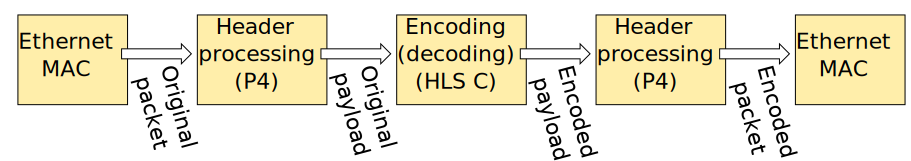
\includegraphics[width=0.4\paperwidth]{Top_level.pdf}
  \caption{\label{fig:toplevel} Block diagram of encoder / decoder pipeline}
\end{figure}

A top-level diagram of the implementation is shown in Fig.~\ref{fig:toplevel}.
Packets arrive on one of the 4 SFP+ cages via a 10Gbps Ethernet cable.
A dedicated 10~Gigabit Transceiver deserializes the packets.  After further
processing by a dedicated Ethernet PHY and in-fabric MAC layer, the entire
packet including Ethernet header is output on a 64-bit AXI Stream bus at 160\,MHz.

The next stage in the pipeline performs packet header preprocessing.  With
ease of implementation and portability in mind, we implemented this in P4, a
domain-specific programming language for packet processing that is target- and
protocol-agnostic \cite{p4_sigcomm_review2014}.  The raw payload, i.e. the frame stripped of Ethernet
header, is forwarded to the FEC core.  \amdrev{The P4 is compiled to FPGA
  logic using Xilinx's SDNet tool suite.}

The FEC core can be an encoder (for the Sending Proxy) or decoder (for the
Receiving Proxy).  In both cases, the FEC core
produces payloads that are the result of, respectively, encoding or decoding
the received group of payloads.  Similar to the header processing, the FEC core
was also created with ease of implementation in mind.  P4 is not suitable
for
\amdrev{payload processing or}
exploiting the parallellism of the FEC core, so we described the core in
hardware-synthesizable C.  As usual, the code can be compiled and executed on a
general-purpose CPU.  More importantly, we can synthesize the code for an FPGA
in Vivado HLS.  Guided by pragmas added by the developer, Vivado HLS takes
advantage of parallelism in the code to achieve a high performance.

The encoded or decoded output of the FEC core feeds into the header
post-processing, which encapsulates the payloads in Ethernet packets.  The
Ethernet subsystem, finally, returns the packets to the network.

\subsection{Header processing}

We use p4 to implement high-level packet processing logic and 

use Xilinx P4-SDNet tool chain to translate p4 program into FPGA and integrate everything together

The translation goes through 3 steps:

First, from P4 to SDNet

Second, from sdnet to RTL implementaion and C++ high-level simulation

Third, add prepheral blocks with Vivado Design Suit

what does P4 do?
Parse packet, modify and tag headers as is described in Design chapter, extract payload for encoder,
control encoder's operation

what is SDNet?
intermediate language, describes the interface, layout, and data flow of data processing engines
at a level closer to RTL modules compared to P4.

\amd{not sure what value the above has -- I do suggest hoisting the SDNet
  comment into the previous section}

%introduce RTL/FPGA?

several challenges:
1. Both P4 and SDNet encourage programs working like a flow - you should never go back and touch anything
a second time. This ensures the efficiency of the program but also makes it harder to express complex
logics. We think it can be a future work to translate a loosely written program into one with such constrains.
Currently we do this manually by keeping in mind a dependency graph of program lines and doing a topological sort
to decide the final order. Using compound operations like
$read\_and\_add\_one$ also helps mitigating this problem.
\amd{I am not following this...and I doubt a reader with no knowledge of
  FPGAs or SDNet will be able to follow either.  What does ``go back'' mean
  in this context? What are you ordering? How is the read-and-add-one
  addressing the problem?}

2. P4 is designed particularly for header processing. There are many
irrelevant \amd{irrelevant is probably not the right word here} things not supported but
necessary in our work, especially payload processing. Most bookkeeping operations can be finished with the
help of external functions like $read\_and\_add\_one$, later implemented in C or Verilog. We also integrate the encoder
into the design by defining an external function for it. However, encoding payload through this interface can be a
great waste for both time and space due to P4's nature of passing and processing a packet as a whole, no matter how long it is. Fortunately, the
flexibility we seek can be found by redirecting SDNet's internal packet flow, which works similar to a 64-bit AXI Stream bus,
to the engine for encoder. This involves modification of less than 10 lines of code per SDNet program, and can be finished by a simple script.
\amd{...don't think this works for a reader either...  Yes, we want to make
the case that P4 doesn't allow payload processing (I suggest adding a note
about that above).  Do we want to dig into the fact that P4 doesn't give us
the expressiveness to stream payload processing, but SDNet does?  ... if
so, we'll need to setup the problem better here and be clearer about the
shape of the solution.}

\subsection{FEC Encoder}

The current implementation is limited to packet encoding, but our intention is
to implement the decoder, too.

Error correction is performed with a Reed-Solomon erasure (RSE) code.  Erasure codes
require prior knowledge of which packets data is missing, as opposed to regular
error correction codes.  This comes with the benefit of requiring fewer error
correction bits.  RSE is a linear code, which means...

\amd{what do we want to highlight here?
  (1) data parallel nature of way FEC RSE is defined ... allows operate on
  the 8 bytes in the 64b per cycle payload independently in data-parallel
  fashion.
  (2) as k scales up, demands more compute...which can address with more
  hardware.
  (3) result is can build hardware to process in a spatial pipeline at the
  160\,MHz data rate necessary to meet 10Gbps link.
  (4) maybe sketch out how much hardware is needed (8$\times$(2+1)$\times$k
  BRAMs)
}

\begin{comment}
Introduce P4.
- Advantages of writing in high-level languages.
- Responsibilities of P4.
- Communication between P4 and encoder
Implementation process
- SDNet
- Vivado HLS
- Vivado
Introduce FPGA.
Top-level design
Matrix multiplication
\end{comment}


\section{Evaluation}
\label{sec:evaluation}
% We evaluate \OurSys using different types of traffic to measure its improvement
% to application-level behavior in the presence of lossy links.

We evaluated \OurSys with microbenchmarks and network simulation.
% to answer these questions:
%\begin{itemize}

%\item What are the resource requirements for \OurSys with different levels of 
%error correction?

%\item How much does \OurSys improve application throughput across lossy links?

%\item What benefit can \OurSys have to networks at large?
%\end{itemize}



% We
% evaluate three possible deployment models for \OurSys: an FPGA external to
% the switch; a software implementation running on the switch CPU; and an ASIC  
% implementation integrated into the switch forwarding engine. 

\subsection{\OurSys models}

\subsubsection{Line Rate P4 Model.} 
To measure the effect of faulty links and
\OurSys at the application level, we implemented a P4 model of lossy links and
the FEC encoder / decoder. The model runs at line  rate alongside the layer 2
forwarding in the Barefoot Tofinos in our  testbed. It captures three
overheads that are important to applications: the bandwidth overhead that the
encoder adds by inserting parity packets and \OurSys headers; the latency
overhead that the decoder adds when recovering lost packets; and the transport
layer overhead that faulty links add by causing packet drops.

\begin{itemize}

\item The \textbf{Encoder Model} encapsulates each packet  egressing on the
faulty link with the \OurSys header and inserts blank  parity packets into the
flow. It tracks per-port block IDs and  packet indices using P4 register
arrays. To generate parity packets, the  model clones the largest packet in
each block with the Tofino's multicast engine. The parity packets are 
delayed until all the data packets in a block egress, using recirculation. 


\item The \textbf{Faulty Link Model} adds a \emph{corruption header} to each packet
egressing the faulty link. The header indicates whether or not the neighbor
switch should consider the packet lost. The model selects packets for corruption
according to a simple binomial distribution implemented with the Tofino's
random number generator.

\item The \textbf{Decoder Model} applies to all packets ingressing from a
modeled faulty link, before any other forwarding logic. For packets that are
not tagged as corrupt, the model simply removes the \OurSys and corruption headers and
allows them to continue to the standard forwarding  pipeline. The model
recirculates corrupt packets until the next block begins, at which point it
decides whether  to recover them based on the number of non-corrupt data and
parity packets it has  observed in the block.  If it counted at least K data
plus parity packets  in the block, the model "recovers" all of the corrupt
packets by removing their corruption headers and forwarding them normally. If
recovery fails, the model simply drops the corrupt packets without forwarding.

\end{itemize}

\begin{figure}
  \centering
  \includegraphics[width=0.3\paperwidth]{figures/lossVsTput.pdf}
  \caption{\label{fig:lossVsTput} Iperf throughput at different loss rates.}
\end{figure}

Figure~\ref{fig:lossVsTput} shows the benefit that FEC has on TCP throughput
at different rates of packet loss, measured with 60 second iperf trials. With
\OurSys, Iperf sustained  over 5 Gb/s with loss up to $10^{-1}$ (1 out of
every 10 packets dropped). Without \OurSys, Iperf's throughput at that loss
rate was under 25 Mb/s.

% This figure shows the impact of H. 

Figure~\ref{fig:lossVsTput} also shows the bandwidth overhead of  FEC, which
is dominated by the number of parity packets per block ($H$).  At loss rates
greater than or equal to $10^{-4}$ the bandwidth overhead of adding  parity
packets had less of an impact on TCP throughput than lost packets, for  most
configurations tested. To reduce bandwidth overhead, the FEC  can be tuned for the
loss rate of each specific link, which is reportedly stable over
time~\cite{corropt}.


% This figure shows the impact of K.
Figure~\ref{fig:lossVsLatency} shows UDP latency statistics ...





\subsubsection{Event-based simulation}
We customised a fat-tree datacenter topology in ns-3~\cite{ns3-dcn} to
model (i)~a link with loss characteristics as described by Zhuo et
al.~\cite{Zhuo:2017:UMP:3098822.3098849}; and (ii)~FEC to support
transport protocols. In this model we experimented with end-to-end
error correction rather than link-layer, to simulate a more complex
implementation without incurring the burden of implementing it fully.

We simulated a 128-node fat-tree network with 10Gbps links where two
nodes communicate over TCP to transfer a 10MB file at 2Gbps. We found
that using FEC completely eliminated retransmissions (which consisted
  of 152, 23, and 2 packets for loss rates of $10^{-3}$, $10^{-4}$,
and $10^{-5}$ respectively). But achieving end-to-end reliability
over a lossy link with little sacrifice to latency came at a steep
end-to-end overhead of 20\%, since a parity packet was added for each
5 data packets. The approach described in this paper only adds
overhead on lossy links, rather than across paths that contain a
lossy link.


\subsection{Encoder Microbenchmarks}
\iffalse
Here we evaluate the implementation directly, not using a model.
Latency and throughput graphs for experiments involving different loss rates, and the encoder working on the CPU and FPGA.
Note: we have not optimized the CPU implementation.
\fi
We measured the performance of our current encoder implementation, which has a
few restrictions.  The encoder parameters are fixed to $k = 8$ and $h = 4$,
and it handles only a single flow of packets with 1024-byte payloads.
Packets were supplied to the FPGA with the packet generator of DPDK 17.08.1.
At the output, we measured a throughput of 9.025 Gbps over a 10-minute period,
nearly saturating the 10-Gbps link.

\iffalse
To ensure \OurSys's effect observed in the model are practical, we directly measured the 
full throughput of our encoder implementation in FPGA. For our benchmark, the encoder is configured to use
k=8 and h=4. Packets are generated by a tool based
on DPDK library, and are fed to the board (as is specified above~(\S\ref{sec:implementation})) through
a 10Gbps link. The average outgoing throughput measured during a 10 minutes test is 9.025Gbps.
Considering the overhead from other parts of the system, we believe the link is actually close
to being saturated, which is our basic assumption in evaluations.
\fi

As a contrast, we also evaluated the CPU implementation (not optimized). Under the same deployment, the throughput measured is 
(\$CPUVALUE), (\$RATIO) lower compared to FPGA.
\lei{TODO: fill the number} \lei{\#Shrink Candidate\#}


\subsection{FPGA resource consumption}
Table~\ref{tab:microbenchmarks} shows the resource requirements for the FPGA implementations of
\OurSys with different $k$ and $h$ parameters.  The resource requirements are
post-implementation utilization values reported by Xilinx Vivado.  We observe
that varying $k$ has a negligible effect on resource consumption, whereas BRAM
consumption has a strong dependence on $h$.  We believe that the BRAM consumption
can be further reduced because several arrays were overpartitioned.
%CPU cycles for the software
%implementation are measured using Linux performance counters and averaged over
%X packets,
%The timing statistics are measured using ingress and egress timestamps on
%the switch.

\iffalse
\begin{table}
% \footnotesize
\begin{center}
\small
% \resizebox{\linewidth}{!}{
\begin{tabular}{ l l l l l l l } 
\toprule
$(k, h)$ & $(25, 1)$ & $(25, 5)$ & $(25,10)$ & $(50, 1)$ & $(50, 5)$ & $(50, 10)$ \\
\midrule
\emph{Software} & & & & & & \\
\cmidrule{1-1}
Cycles & & & & & & \\
Proc. Time (ns) & & & & & & \\
\midrule
\emph{FPGA} & & & & & & \\
\cmidrule{1-1}
BRAM (18Kb) & 135 (7\%) & 186 (10\%) & 248 (14\%) & 135 (7\%) & 186 (10\%) & 248 (14\%) \\
DSP & 0 (0\%) & 0 (0\%) & 0 (0\%) & 0 (0\%) & 0 (0\%) & 0 (0\%) \\
Flip-flop & 52420 (10\%) & 53415 (10\%) & 54497 (10\%) & 52420 (10\%) & 53416 (10\%) & 54496 (10\%) \\
LUT & 31372 (11\%) & 32439 (12\%) & 33136 (12\%) & 31368 (11\%) & 32479 (12\%) & 33215 (12\%) \\
Proc. Time (ns) & & & & & & \\
\bottomrule
\end{tabular}
% }
\caption{Resource requirements for FPGA and CPU implementations of \OurSys with different configurations.}
\label{tab:microbenchmarks}
\end{center}
\end{table}
\fi

\begin{table}
% \footnotesize
\begin{center}
\small
% \resizebox{\linewidth}{!}{
\begin{tabular}{ l r r r r } 
\toprule
$(k, h)$ & $(25, 1)$ & $(25, 5)$ & $(25,10)$ & $(50, 1)$ \\
\midrule
%\emph{Software} & & & & \\
%\cmidrule{1-1}
%Cycles & & & & \\
%Proc. Time (ns) & & & & \\
%\midrule
%\emph{FPGA} & & & & \\
%\cmidrule{1-1}
BRAM (18Kb) & 135 (7\%) & 186 (10\%) & 248 (14\%) & 135 (7\%) \\
DSP & 0 (0\%) & 0 (0\%) & 0 (0\%) & 0 (0\%) \\
Flip-flop & 52420 (10\%) & 53415 (10\%) & 54497 (10\%) & 52420 (10\%) \\
LUT & 31372 (11\%) & 32439 (12\%) & 33136 (12\%) & 31368 (11\%) \\
%Proc. Time (ns) & \FIXME{?} & & & \\
\bottomrule
\end{tabular}
% }
\caption{Resource and Performance measurement %Comparison
of the FPGA %and CPU
implementation of \OurSys with different configurations.}
\label{tab:microbenchmarks}
\end{center}
\end{table}

%We run \OurSys in 3 configurations: outside the switch, on the switch, and in the switch.
%Time how quickly \OurSys reacts to failing links.

\section{Conclusion}
In this paper we described \OurSys, a new in-network mitigation
against failing network links. It monitors network ports to infer
abnormal loss, and uses forward error-correction across lossy links.
Adjacent switches coordinate to set up complementary encoding and
decoding stages for FEC across failing links.  We prototyped the FEC
encoding and decoding stages on x86 systems for ease of development
and also prototyped the encoding stage to run on reconfigurable
hardware.

Our implementation is a work in progress, and we are extending it to
carry out the decoding stage on reconfigurable hardware, too.
Another improvement consists of using all the network ports on our
development board and scaling up our testing to use all available
bandwidth.
Finally, we will add the configuration and coordination logic to
specify traffic classes and the parameters to the FEC.

We also plan to extend this work further to explore autonomous
network resource management, going beyond in-network mitigation of
faulty links. We will explore in-network services that require
a level of programmability that exceeds P4's current capabilities,
such as data deduplication and compression and build on the system
described in this paper.


\subsection*{Acknowledgements}
This material is based upon work supported by the Defense Advanced
Research Projects Agency (DARPA) under Contract No. HR001117C0047.
Xilinx provided tools and IP, including SDNet to support P4 to FPGA
compilation, the Ethernet MAC, and HLS and physical design mapping
software. 

\bibliographystyle{ACM-Reference-Format}
\bibliography{paper}

\end{document}
